% Created 2017-09-21 Thu 22:33
% Intended LaTeX compiler: pdflatex
\documentclass[setspace, doublespace]{scrartcl}
\usepackage[utf8]{inputenc}
\usepackage[T1]{fontenc}
\usepackage{graphicx}
\usepackage{grffile}
\usepackage{longtable}
\usepackage{wrapfig}
\usepackage{rotating}
\usepackage[normalem]{ulem}
\usepackage{amsmath}
\usepackage{textcomp}
\usepackage{amssymb}
\usepackage{capt-of}
\usepackage{hyperref}
\usepackage{indentfirst}
\setlength{\parindent}{2em}
\setlength{\parskip}{1em}
\author{Xiong ChenYu \\
U1521516C \\
EEE \\
}
\date{Sep 19, 2017 \\
}
\title{
\includegraphics[width=\textwidth]{img/NTU.png} \\
[3\baselineskip] REPORT \\
ON \\
ASSIGNMENT 1 \\
[5\baselineskip]}
\hypersetup{
 pdfauthor={Xiong ChenYu \\
U1521516C \\
EEE \\
},
 pdftitle={
\includegraphics[width=\textwidth]{img/NTU.png} \\
[3\baselineskip] REPORT \\
ON \\
ASSIGNMENT 1 \\
[5\baselineskip]},
 pdfkeywords={},
 pdfsubject={},
 pdfcreator={Emacs 27.0.50 (Org mode 9.1.1)},
 pdflang={English}}
\begin{document}

\maketitle
\tableofcontents

\newpage
\section{Abstract}
\label{sec:orgf6d0c21}
This report answer questions of the research and study on the assignment 1
which is the numerical analysis of the \(x^{\frac{1}{3}}\). Each
Question answer section consist of 2 part consist of 2 part. First part is the
use of bisection method and the second part is the use of Newton's method. And
the conclusion is the comparison of the two method.

\newpage
\section{Question 1 (my strategy)}
\label{sec:org611d34d}
To solve the problem. I need to define a recursive function to get the better
and better precision. And a end condition predicate to stop the recursive call.
The end condition is the same, so I need to choose 2 different kind of
recursive method to approximate the real value.

\subsection{Bisection Method}
\label{sec:orgf0e7c24}
This method come into my mind cause we learn how to solve the square root in
the tutorial. So I came about a similar idea to carry out this method.

This is the mathematics is topology like a binary search tree. Trying to
narrow the interval of the answer area by repeatedly bisecting and comparing.

\subsection{Newton's Method}
\label{sec:org94941a1}
And this one is what we learn in the year 2 math class. Chapter numerical
method. We use Tyler series to drive the convergence rate of this method.

In numerical analysis, Newton's method (also known as the Newton–Raphson
method), named after Isaac Newton and Joseph Raphson, is a method for finding
successively better approximations to the roots (or zeroes) of a real-valued
function. It is one example of a root-finding algorithm.


\section{Question 2}
\label{sec:orgeaa0ad0}
let \(x^{\frac{1}{3}}\) = t, so the questions is equivalent to \(y = x^3 -t\)
\subsection{Bisection Method}
\label{sec:org550bdc6}
In bisecting method the upper bound and the lower bound with define in
Haskell type class Range, and we have 5 conditions and we have to define the
upper and lower bounder separately.

The range can be classified into 5 sub-
range:(\(-\infty\),-1),[-1,0),[0],(0,1],(1,\(\infty^+\))

Since it is symmetric, let us talk about the positive range of it.

If x > 1, the lower border is obvious to be 1, and the upper range is \(\frac{(x + 1)}{2}\).
$$(\frac{(x + 1)}{2})^3 / x = \frac{x^3 + 3(x^2)+3x+1}{8} / x =  \frac{x^3 + 3(x^2)+3x+1}{8x}$$

since \(x^3 >= 1, x^2 >=1 ,x>=1\), so \(\frac{x^3 + 3(x^2)+3x+1}{8x} >=0\), so
max border is upper than x\(_{\text{ans}}\).

If \(0<x<=1\), the lower bounder is obvious to be 0, and the upper range is x
since \(x<1\) ,so \(x^3 < x\).

And x = 0 is obvious to be zero.

While in all range, we narrow our range to be half, so the answer series is converge.

\begin{center}
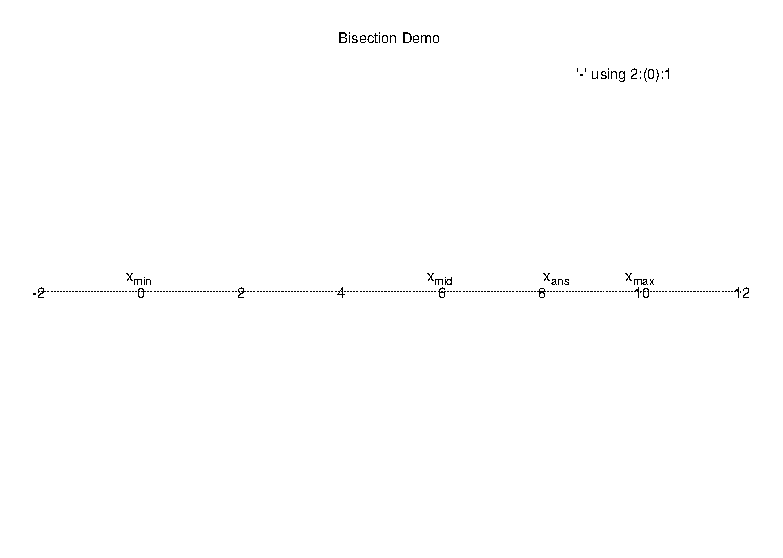
\includegraphics[width=.9\linewidth]{test.eps}
\end{center}

\subsection{Newton's Method}
\label{sec:org42f2a0f}

The Newton–Raphson method in one variable is implemented as follows:

The method starts with a function f defined over the real numbers x, the
function's derivative \(f′\), and an initial guess x\(_{\text{0}}\) for a root of the
function f.

If the function satisfies the assumptions made in the derivation of the formula
and the initial guess is close, then a better approximation x\(_{\text{1}}\) is
$$ x_1 = x_0 - \frac{f(x_0)}{f'(x_0)} $$

Geometrically, (x\(_{\text{1}}\), 0) is the intersection of the x-axis and the tangent of
the graph of \(f\) at (x\(_{\text{0}}\), \(f (x_0)\)).
The process is repeated as
$$ x_{n+1} = x_n - \frac{f(x_n)}{f'(x_n)} $$

For the correctness of Newton's Method all we need to ensure is 2 part:
$$ f'x = 3x^2$$
So when x = 0,\(f'x = 0\), I use pattern matching to just return the 0 value to avoid the
NaN happens.
$$ f''x = 6x $$
So it is a monotone increasing function. The tangent line and x-xies is
converge.
That prove the newton's method is always correct in my code.

\section{Question 3}
\label{sec:org6f0c2e1}
\subsection{Bisection Method}
\label{sec:org7073cc9}
We can analysis this method by complexity and convergence rate.
\subsubsection{Complexity}
\label{sec:org35617c2}
When the precision is fixed. And the value of n become infinity. The
complexity of the bisection method is \(log_2(x)\)
\subsubsection{Convergence Rate}
\label{sec:orgd3e6cc2}
When the number of precision digit is fixed we can see that:
$$ \frac{precision - x_{n+1}}{precision - x_{n}} = \frac{1}{2} $$
So the convergence rate of bisection method is linear to be n.

\subsection{Newton's Method}
\label{sec:orgf5f5c23}
\subsubsection{Complexity}
\label{sec:orgd0fedc3}
When the precision is fixed. And the value of n become infinity.It is hard to
define the complexity of the newton's Method. Because newton's method is
greatly affected by the initial guess value. So we can not find the worst
case. Cause if you define a worst case initial value x\(_{\text{worst}}\) there must exist
a even worst value:
$$ x_{worst} = x_{evenworst} - \frac{f(x_{evenworst})}{f'(x_{evenworst})} $$
So it is a np problem. The complexity of the Newton's is log\(_{\text{2}}\)(x).
\subsubsection{Convergence Rate}
\label{sec:org17d1b81}
By use of Tyler series we can easily prove.
$$f(\alpa) = f(x_n) + f'(x_n)(\alpha - x_n) + R_1$$
$$R_1 - \frac{1}{2!}f''(\beta_n)(\alpha - x_n)$$
since \(\alpha\) is the root, So we have:
$$0=f(\alpha) = f(x_n) + f'(x_n)(\alpha - x_n) +
    \frac{1}{2}f''(\beta_n)(\alpha - x_n)^2$$
$$\underbrace{\alpha-x_{n+1}}_{\beta_{n+1}} =
    \frac{-f''(\beta)}{2f'(x_n)}(\alpha-x_n)^2$$
Therefor \(error_{n+1} = error_n^2\)
So the convergence rate of newton's method is quadratic.
\section{Conclusion}
\label{sec:org2189a49}
Even the complexity of the 2 method is nearly the same. While the newton's
method have the higher convergence rate. So I suggest to use the newton's
method.
\end{document}